% AKULIN--KARLOV, Fig. 20.2. CP09, source-traced ink reconstruction.
% Pixel-space control points are EDITORIAL TRACING of the 752 x 575 original.
% This is a qualitative cusp catastrophe, NOT numerical data or a fitted model.
% Geometric invariants: A is the cusp point; C/B are opposite switching folds;
% two diagonal dashed guides and independent inner-left sheet edge are retained.
\documentclass[border=6pt]{standalone}
\usepackage{fontspec,unicode-math}
\setmainfont{Noto Serif}
\setmathfont{STIXTwoMath-Regular.otf}
\usepackage{tikz}
\usetikzlibrary{arrows.meta,calc}
\tikzset{
 axis/.style={draw=black,line width=.70pt,-{Latex[length=2.3mm,width=1.3mm]}},
 sheet/.style={draw=black,line width=1.36pt,line cap=round,line join=round},
 folded/.style={draw=black,line width=1.55pt,line cap=round,line join=round},
 guide/.style={draw=black,line width=.66pt,dash pattern=on 4.0pt off 3pt},
 hatchline/.style={draw=black,line width=.51pt},
 lab/.style={font=\fontsize{12}{14}\selectfont,inner sep=1.1pt},
 tinylabel/.style={font=\fontsize{10.8}{13}\selectfont,inner sep=.8pt}}
\begin{document}
\begin{tikzpicture}[x=.016cm,y=-.016cm]
\path[use as bounding box] (0,0) rectangle (751,573);
% Main projected T_x, I, and fractional concentration axes.
\draw[axis] (168,310)--(740,314);
\draw[axis] (168,310)--(168,9);
\draw[axis] (168,310)--(309,559);
\node[lab,anchor=west] at (701,345) {$T_{\mathrm{x}}$};
\node[lab,anchor=west] at (311,545) {$I$};
\node[lab,anchor=west] at (211,26) {$\dfrac{n_B}{n_A+n_B}$};
% Exterior upper fold: its upper ridge and right descending edge (same original vertices).
\draw[sheet] (168,310) .. controls (238,283) and (332,266) .. (370,226)
 .. controls (410,189) and (406,131) .. (474,86)
 .. controls (504,63) and (528,50) .. (537,44)
 .. controls (593,88) and (675,164) .. (720,224);
% Outer lower boundary and the oblique front-left edge.
\draw[sheet] (168,310)--(283,515);
\draw[sheet] (283,515)--(720,224);
% Author's exposed internal seam starts at (210,417), NOT on the left oblique edge.
% Keep this open start: CP07 had incorrectly welded it to the exterior face.
\draw[sheet] (210,416) .. controls (272,391) and (379,347) .. (419,303)
 .. controls (436,288) and (438,269) .. (448,246)
 .. controls (458,207) and (483,184) .. (510,170)
 .. controls (549,149) and (596,140) .. (628,128);
% Folded multivalued sheet: C is the upper turning point and B is lower-right.
\draw[folded] (439,281) .. controls (447,314) and (458,359) .. (475,361)
 .. controls (498,359) and (524,347) .. (531,370)
 .. controls (539,392) and (508,400) .. (479,420);
% Other fold return to the cusp A, then the downward sheet tail.
\draw[folded] (439,281) .. controls (437,333) and (421,359) .. (440,388)
 .. controls (465,430) and (536,463) .. (604,478);
% Sheet branch beneath the forward rim (this branch is distinct from the author seam).
\draw[sheet] (283,515) .. controls (355,483) and (461,425) .. (528,383);
% Author's projection guides: two horizontals, vertical, and BOTH slanted fold guides.
\draw[guide] (170,311)--(440,313);
\draw[guide] (205,385)--(440,386);
\draw[guide] (439,280)--(439,391);
\draw[guide] (389,337)--(440,389);
\draw[guide] (439,281)--(501,340);
% Author's oblique shaded two-parameter multistability region.
% Only TWO black boundaries are explicitly drawn in the scan; the free hatch ends
% are not connected by a spurious third boundary (the CP09 prototype did so).
\begin{scope}
  \clip (440,389)--(504,529) -- (604,478)
     .. controls (543,463) and (468,427) .. cycle;
  \foreach \i in {1,...,23} {
    \pgfmathsetmacro{\t}{\i/24}
    \draw[hatchline] ({440+64*\t},{389+140*\t}) --
       ({440+164*\t},{389+178*\t-89*\t*\t});
  }
\end{scope}
\draw[hatchline] (440,389)--(504,529);
% Labels close to their ORIGINAL branch (never labels as new graph vertices).
\node[lab,anchor=west] at (451,350) {$C$};
\node[lab,anchor=north east] at (429,391) {$A$};
\node[lab,anchor=west] at (538,378) {$B$};
% Hysteresis inset: two stable branches, different switching temperatures.
\draw[axis] (15,521)--(209,521);
\draw[axis] (15,521)--(15,346);
\node[tinylabel,anchor=west] at (28,341) {$\dfrac{n_B}{n_A+n_B}$};
\node[lab,anchor=west] at (181,547) {$T_{\mathrm{x}}$};
\draw[sheet] (49,503) .. controls (89,495) and (129,480) .. (130,456)
 .. controls (130,438) and (104,436) .. (79,429)
 .. controls (47,420) and (55,401) .. (87,387)
 .. controls (105,379) and (123,376) .. (140,376);
\draw[axis] (60,433)--(60,484); % cooling: C -> lower branch
\draw[axis] (132,447)--(132,380); % heating: B -> upper branch
\node[lab,anchor=east] at (56,414) {$C$};
\node[lab,anchor=west] at (135,455) {$B$};
\end{tikzpicture}
\end{document}
